\section{Data analysis}

Data were preprocessed with the three software packages: Elekta Neuromag\textsuperscript{\textregistered} MaxFilter (version 2.2, \cite{3.3.MNE}), Matlab (version 2014a) and MNE-Python (version 0.8.6, \cite{3.3.MNEpython}).

\subsection{Behavioral data}

Two types of behavioral data were analyzed for group and condition effects: response time (RT) and response accuracy (RA).
Response time was measured at the condition onset, i.e. at the "'d"' sound of "'den"' or "'der"' (in the subject-relative clause or the object-relative clause, respectively).
Trials were omitted when the subject skipped or answered them incorrectly.
Trials were also omitted if the response took longer than 4000ms.
This procedure removed 11.1\% of the childrens' trials, and 2.5\% of the adults' trials.

RT and RA were determined for each subject separately from the remaining trials.
Both metrics were tested for the requirements for an analysis of variance (ANOVA).
Normality of the residuals was tested with a Shapiro-Wilk test \cite{3.3.swtest}, implemented in Matlab.
Equality of variances was tested with a Levene test\cite{3.3.levtest}, implemented in SPSS.
RA data failed the normality test.
To include RA data in the following analysis, they were transformed to fit a normal distribution.
This transformation was accomplished with the inverted sigmoid function:
\[ \hat{a} = - log( \frac{1}{a} - 1 ) \]
All results from the ANOVA were transformed back into milisecond space with the sigmoid function:
\[ r = \frac{1}{1+e^{-\hat{r}}} \]


\subsection{Sensor-space activity}

\paragraph{Preprocessing and HPI correction}
Signal-space separation \cite{3.3.SSS} was used to reduce noise in the data by suppressing magnetic interference coming from outside and inside the sensory array.
MEG recordings were corrected for HPI movements, and co-registered across blocks to the inital head position for each individual.
All of these steps were computed with MaxFilter.
Data were then subjected to a 0.4Hz FIR highpass filter (Hamming window design, 4367 coefficients, -130db suppression at 0Hz, -3db at 0.4Hz,processing in Matlab) to remove slow trends.

\paragraph{Artifact removal}
MEG channels with abnormally high noise levels as identified by visual inspection were rejected from further analysis. A median of 1 channel (maximum: 3 channels) was removed.
The resulting pre-processed data contained major artifacts from spontaneous channel jumps, electrocardiographic (ECG) activity and electrooculographic (EOG) activity.
Jump amplitudes were detected by selecting peaks in the z-transformed continuous data that exceeded a threshold of 12 standard deviations.
Segments of 2 seconds in the pre-processed continuous data were rejected if any magnitude channel exceeded an amplitude of $6\cdot10^{-12}T$ (gradiometer channels: $4\cdot10^{-12}\frac{T}{cm}$).
Continuous data were then decomposed into independent components (ICA) that explained 99\% of the variance.
Components that correlated with EOG or ECG channels were removed with the MNE functions \emph{preprocessing.ica\_find\_ecg\_events()} and \emph{preprocessing.ica\_find\_eog\_events()}, respectively.
ICA-based correction removed an average of 2.1 components per subject and block (minimum: 1, maximum: 4).
The remaining ICA components were used to reconstruct continuous data.

\paragraph{Epoching}
The main trigger was set at the condition onset (described in section 3.1.4).
Epochs were created between 1000ms before and 4000ms after the main trigger.
An epoch was rejected if the trial was skipped, or answered too slow (more than 4000ms) or answered incorrectly.
This procedure yielded an average of [] trials in children and [] trials in adults.
Data were filtered before epoching with a 45Hz FIR lowpass (using the MNE function \emph{raw.filter()}) exclusively for the following two steps.

\paragraph{Cluster analysis}
The condition effect was used to determine suitable time windows.
Selecting data purely based on contrast will include spurious differences as well as the condition-based differences in activity.
Since there the subsequent statistical analysis compares the same contrast, it is prone to overestimate the condition effect.
This problem was resolved with a cluster-level permutation comparison.
Spurious differences in activity should vary randomly between trials and subjects, while the condition contrast is expected with a roughly equal delay and duration.

One pair of trials was pooled for each syntax condition over all trials in a group.
Each trial consisted of mean activity from one of each of three sensor groups (from parietal, temporal and frontal locations).
Clusters were computed by running the MNE function \emph{stats.permutation\_cluster\_test()} \cite{3.3.clustertest} over the pair of trials.
The function was run with 2500 permutations, and an t-threshold of 2.0.
Since the group had a strong impact on RT (see [4.1.1]), effective time windows were estimated separately for children and adults.

\paragraph{Interval analysis}
Additionally, a blind comparison was performed for sensor activity in a series of time intervals.
10 time intervals were established from 0ms to 2200ms\footnote{As determined in the following analysis of response times, these intervals cover 95\% of childrens' trials completely, and 98\% of the adults'.} after onset, spanning 200ms each.
The mean sensor activity was computed for each sensor group (3), hemisphere (2), time interval (10), yielding 60 activity values for each subject and condition.
The corresponding values were pooled over all subjects within each of the two groups, and compared between syntax conditions with a paired Student's T-test.
Results from each hemisphere and sensor group were adjusted with the false discovery rate correction (10 comparisons).

For visualization purposes, grand average activity was also calculated for each sensor group and condition, separately for children and adults.

\begin{figure}[h]
\begin{center}
\vspace{7mm}
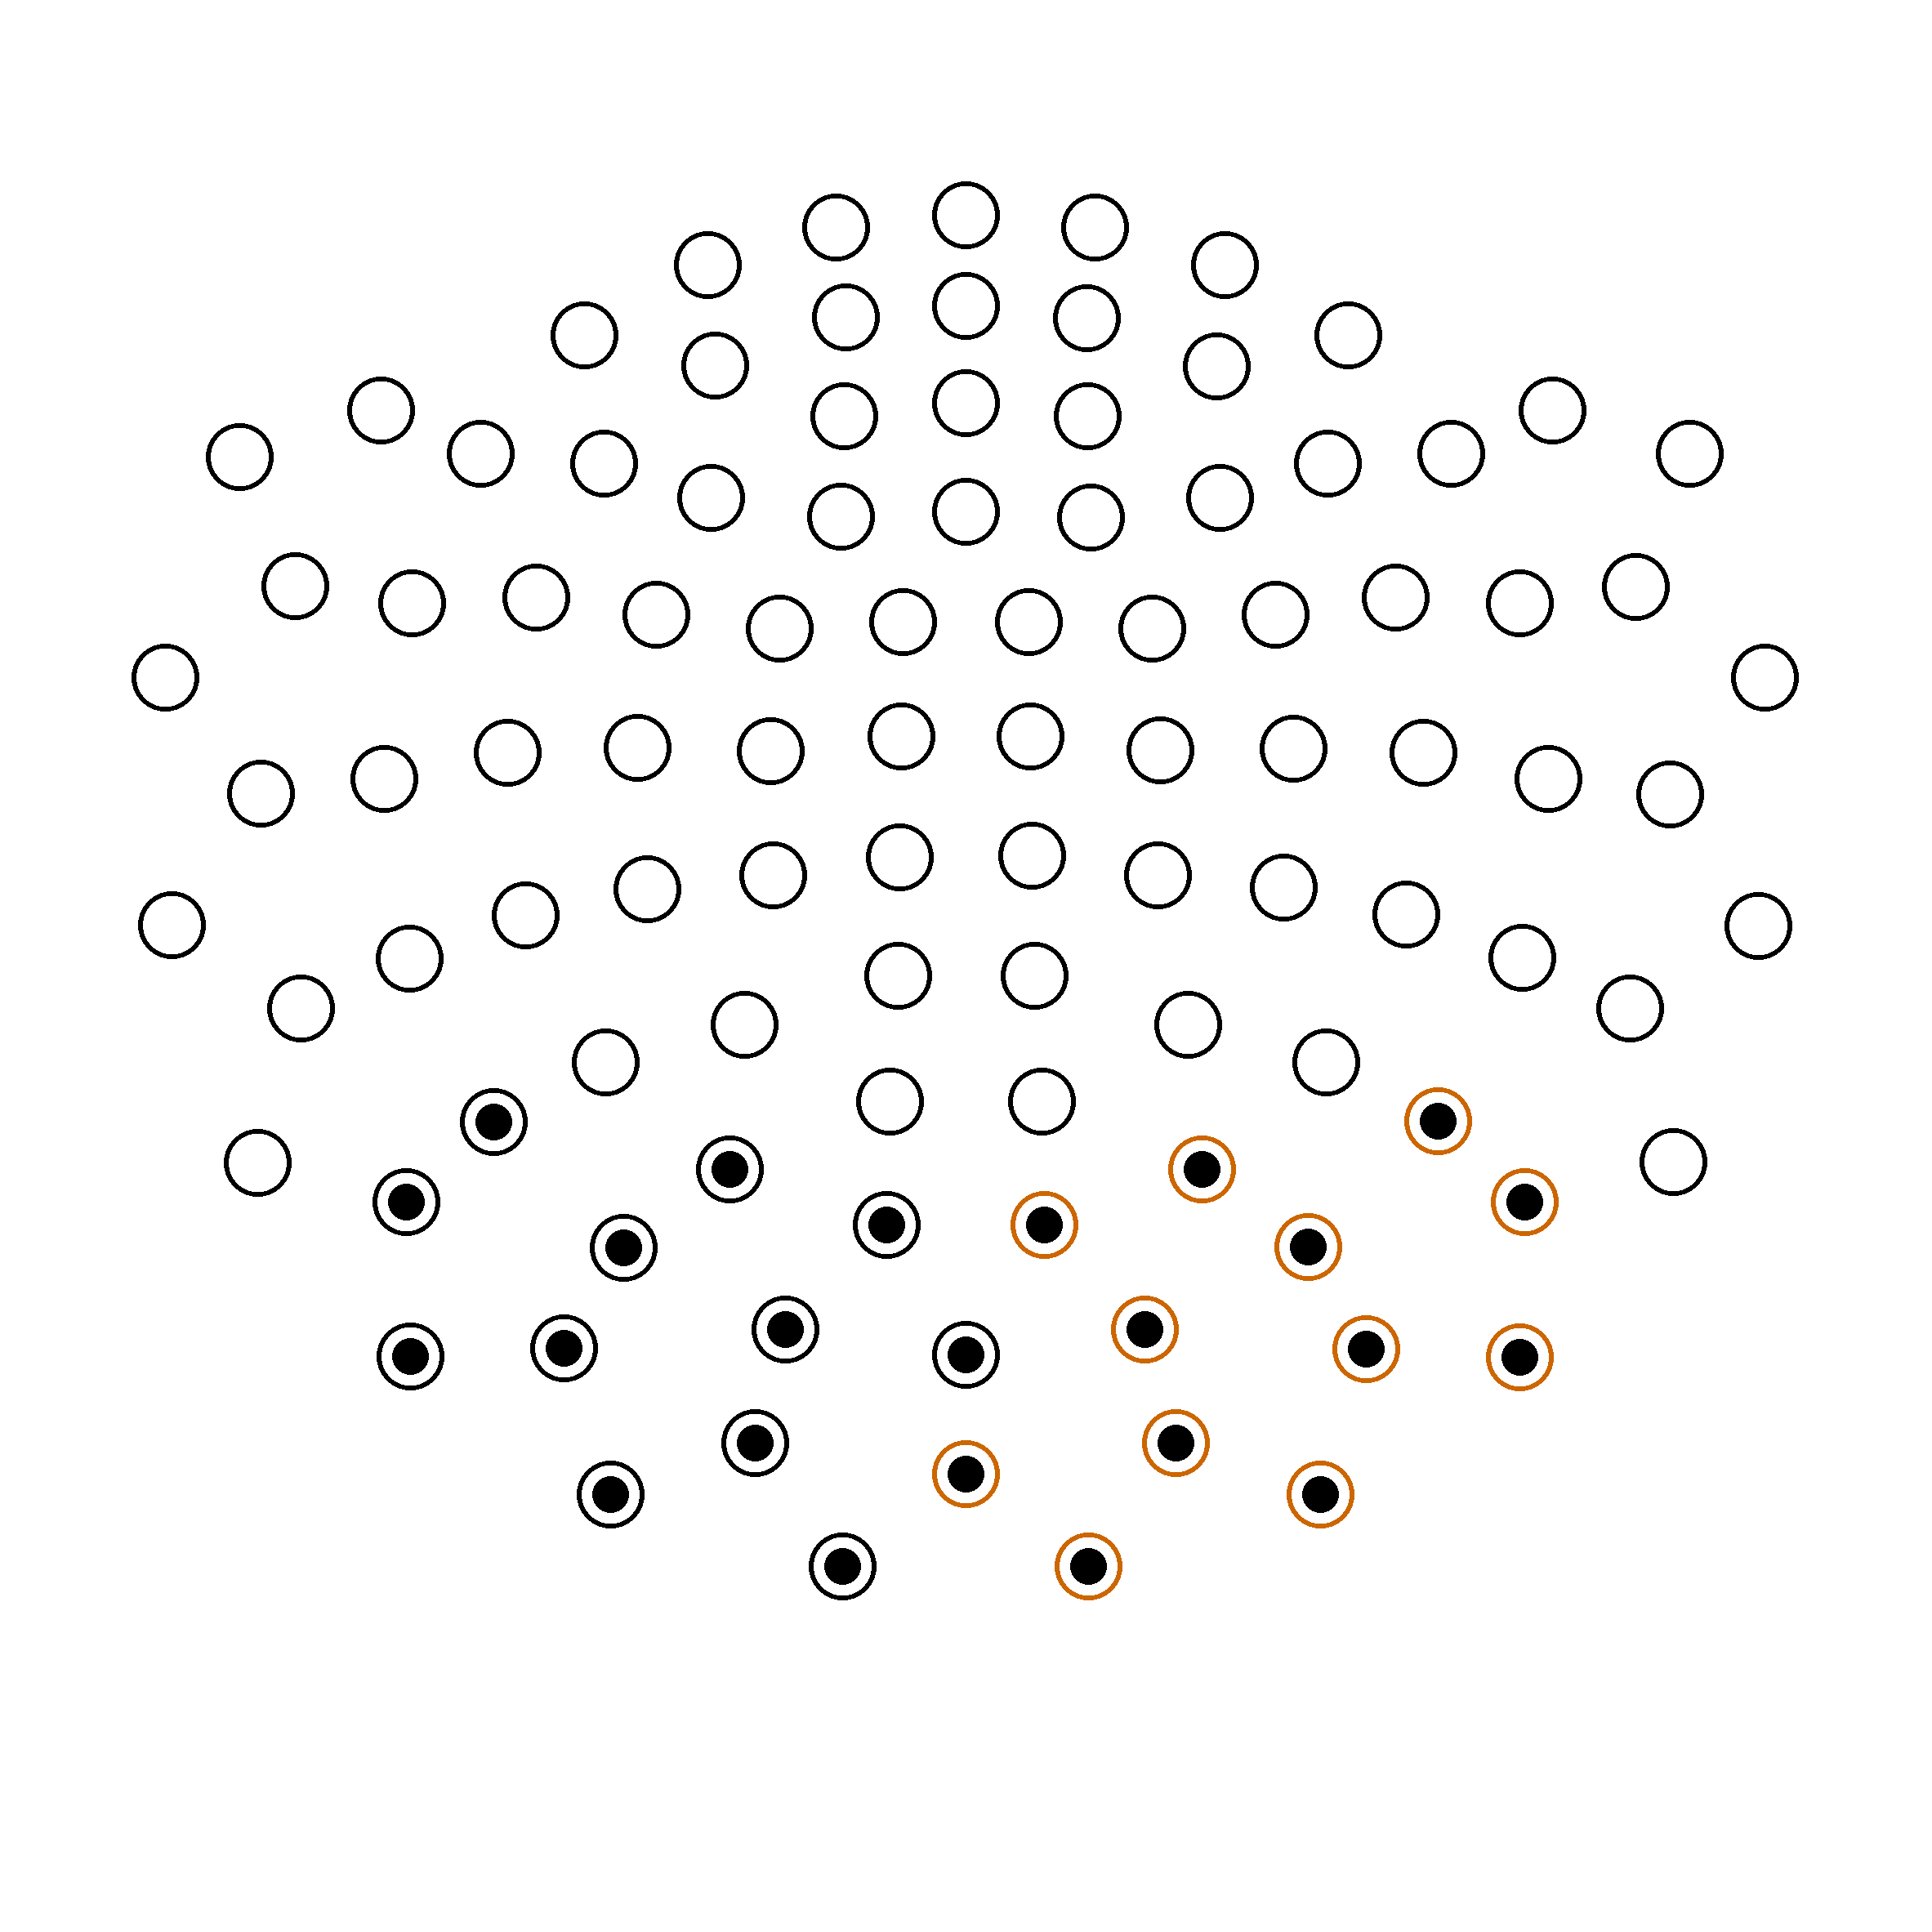
\includegraphics[width=0.24\textwidth]{pics/3_3_occipital_sensors}
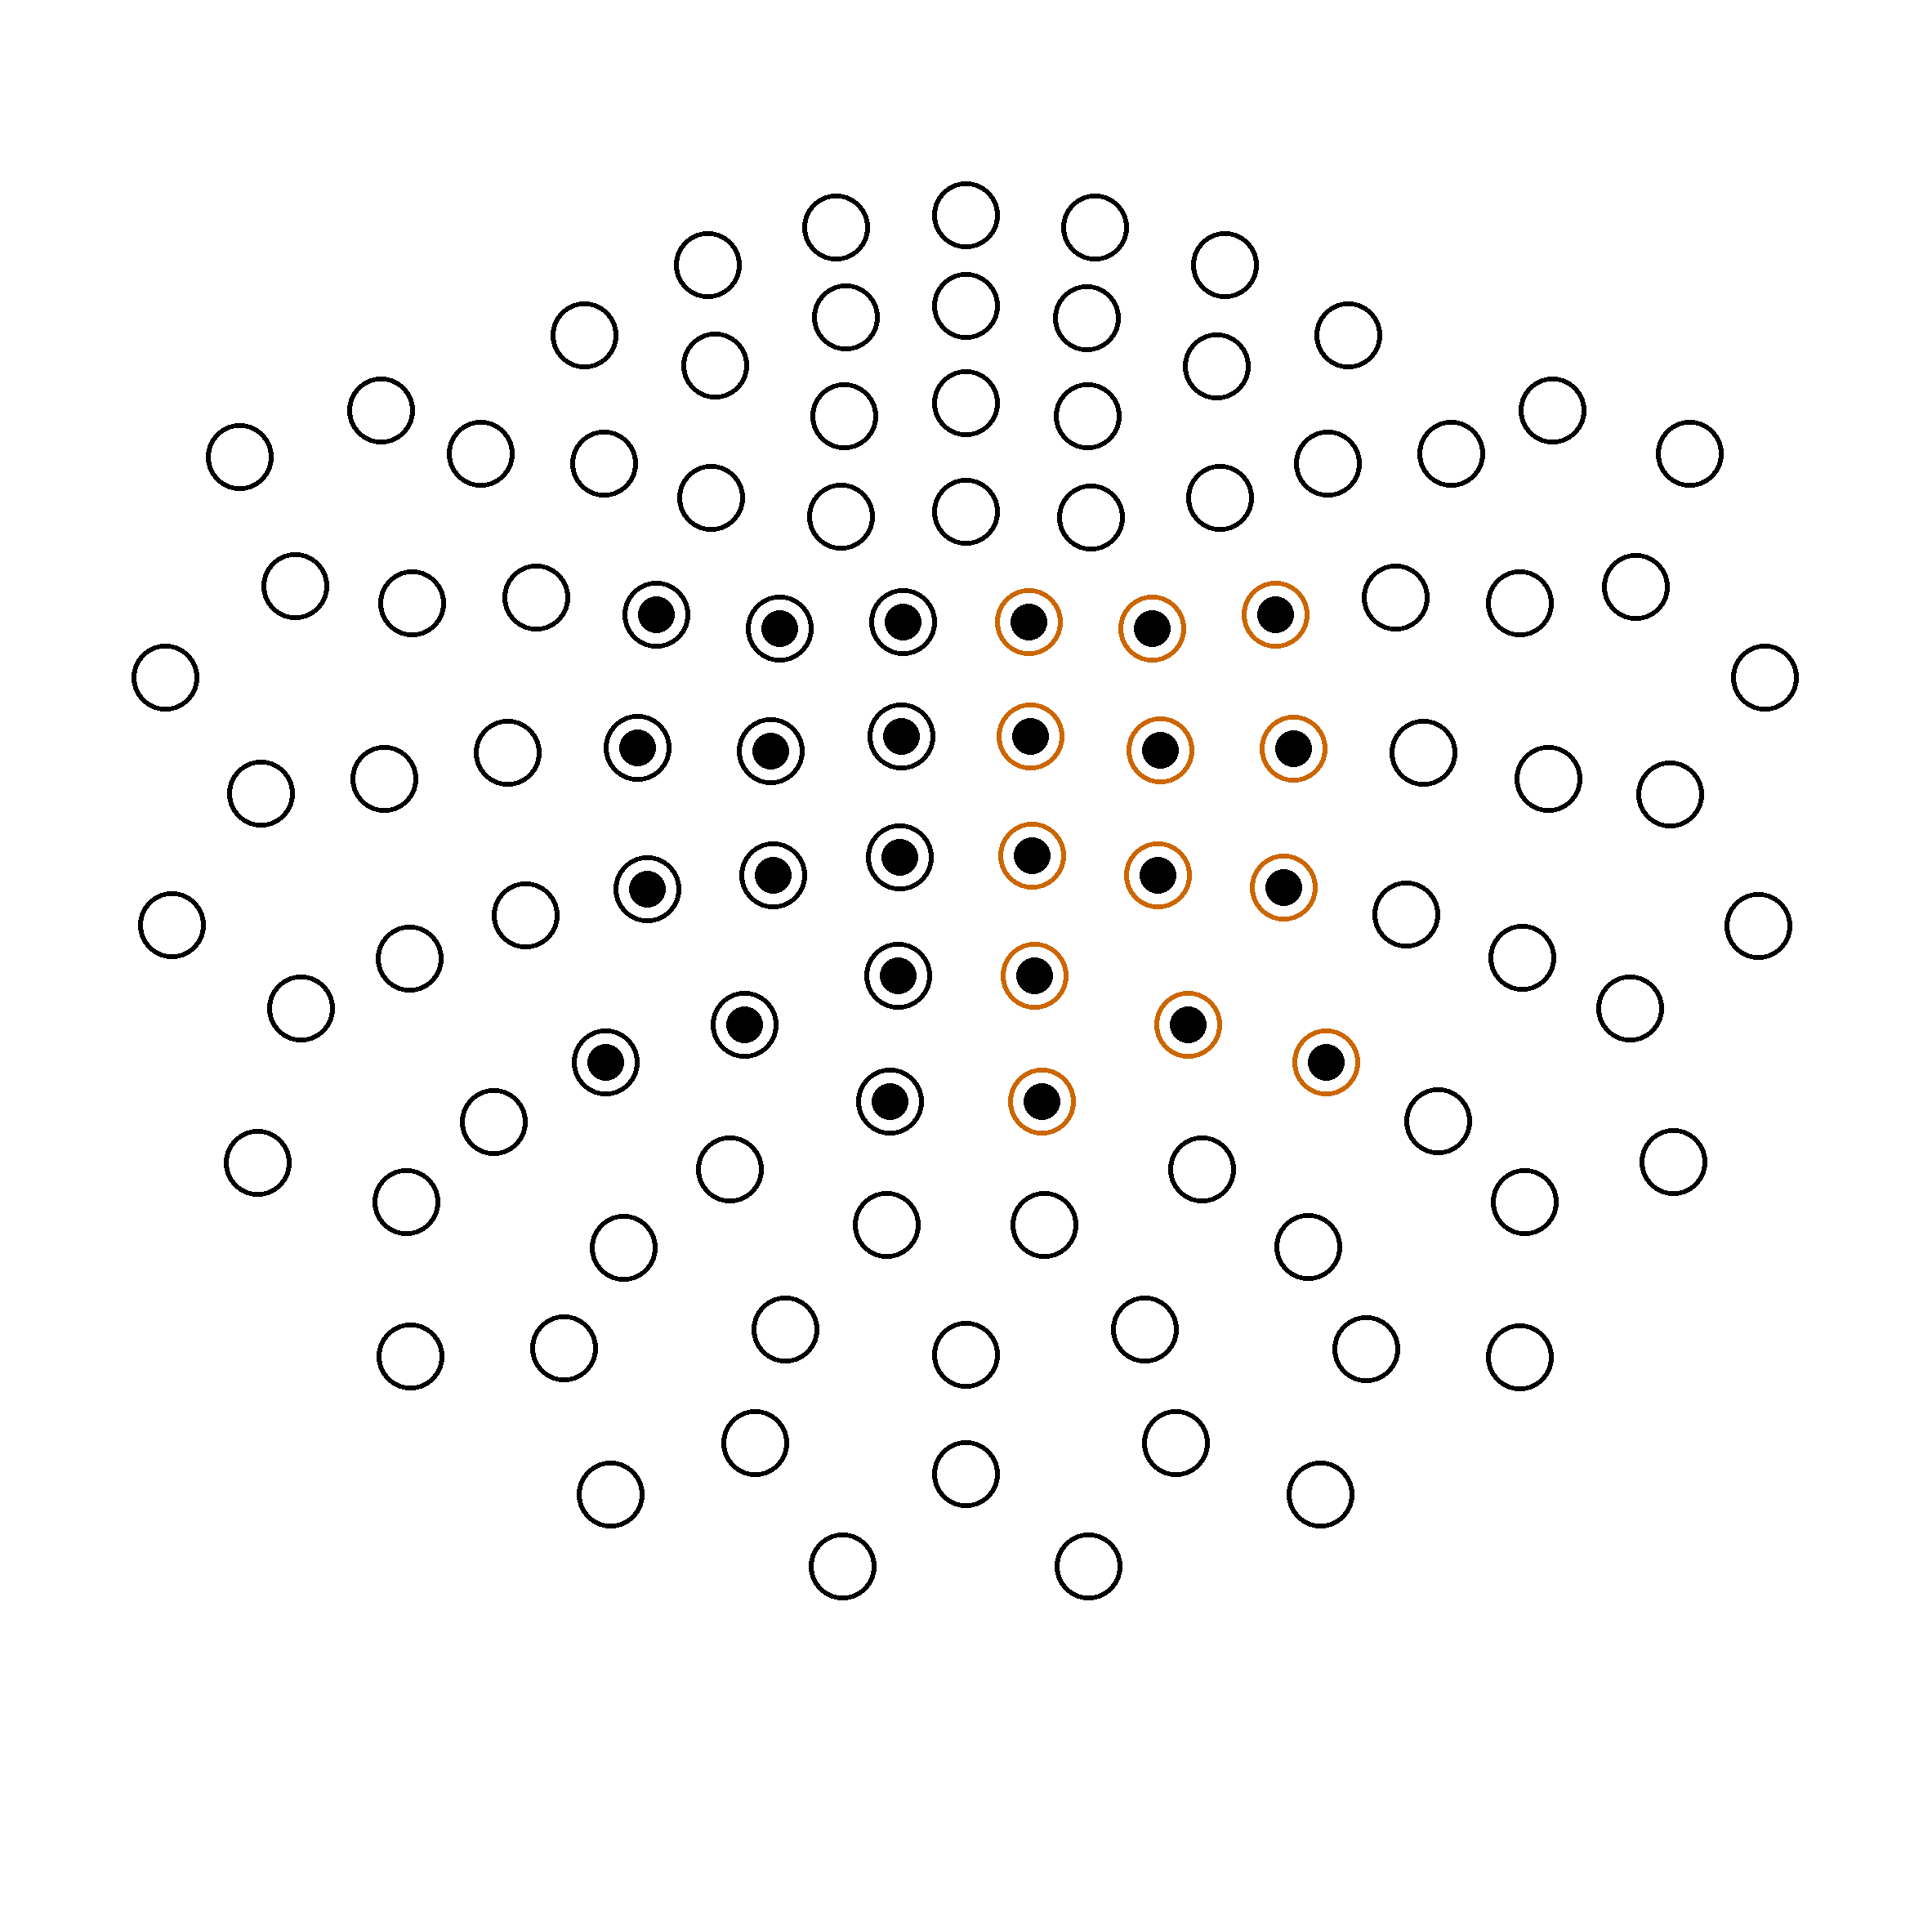
\includegraphics[width=0.24\textwidth]{pics/3_3_parietal_sensors}
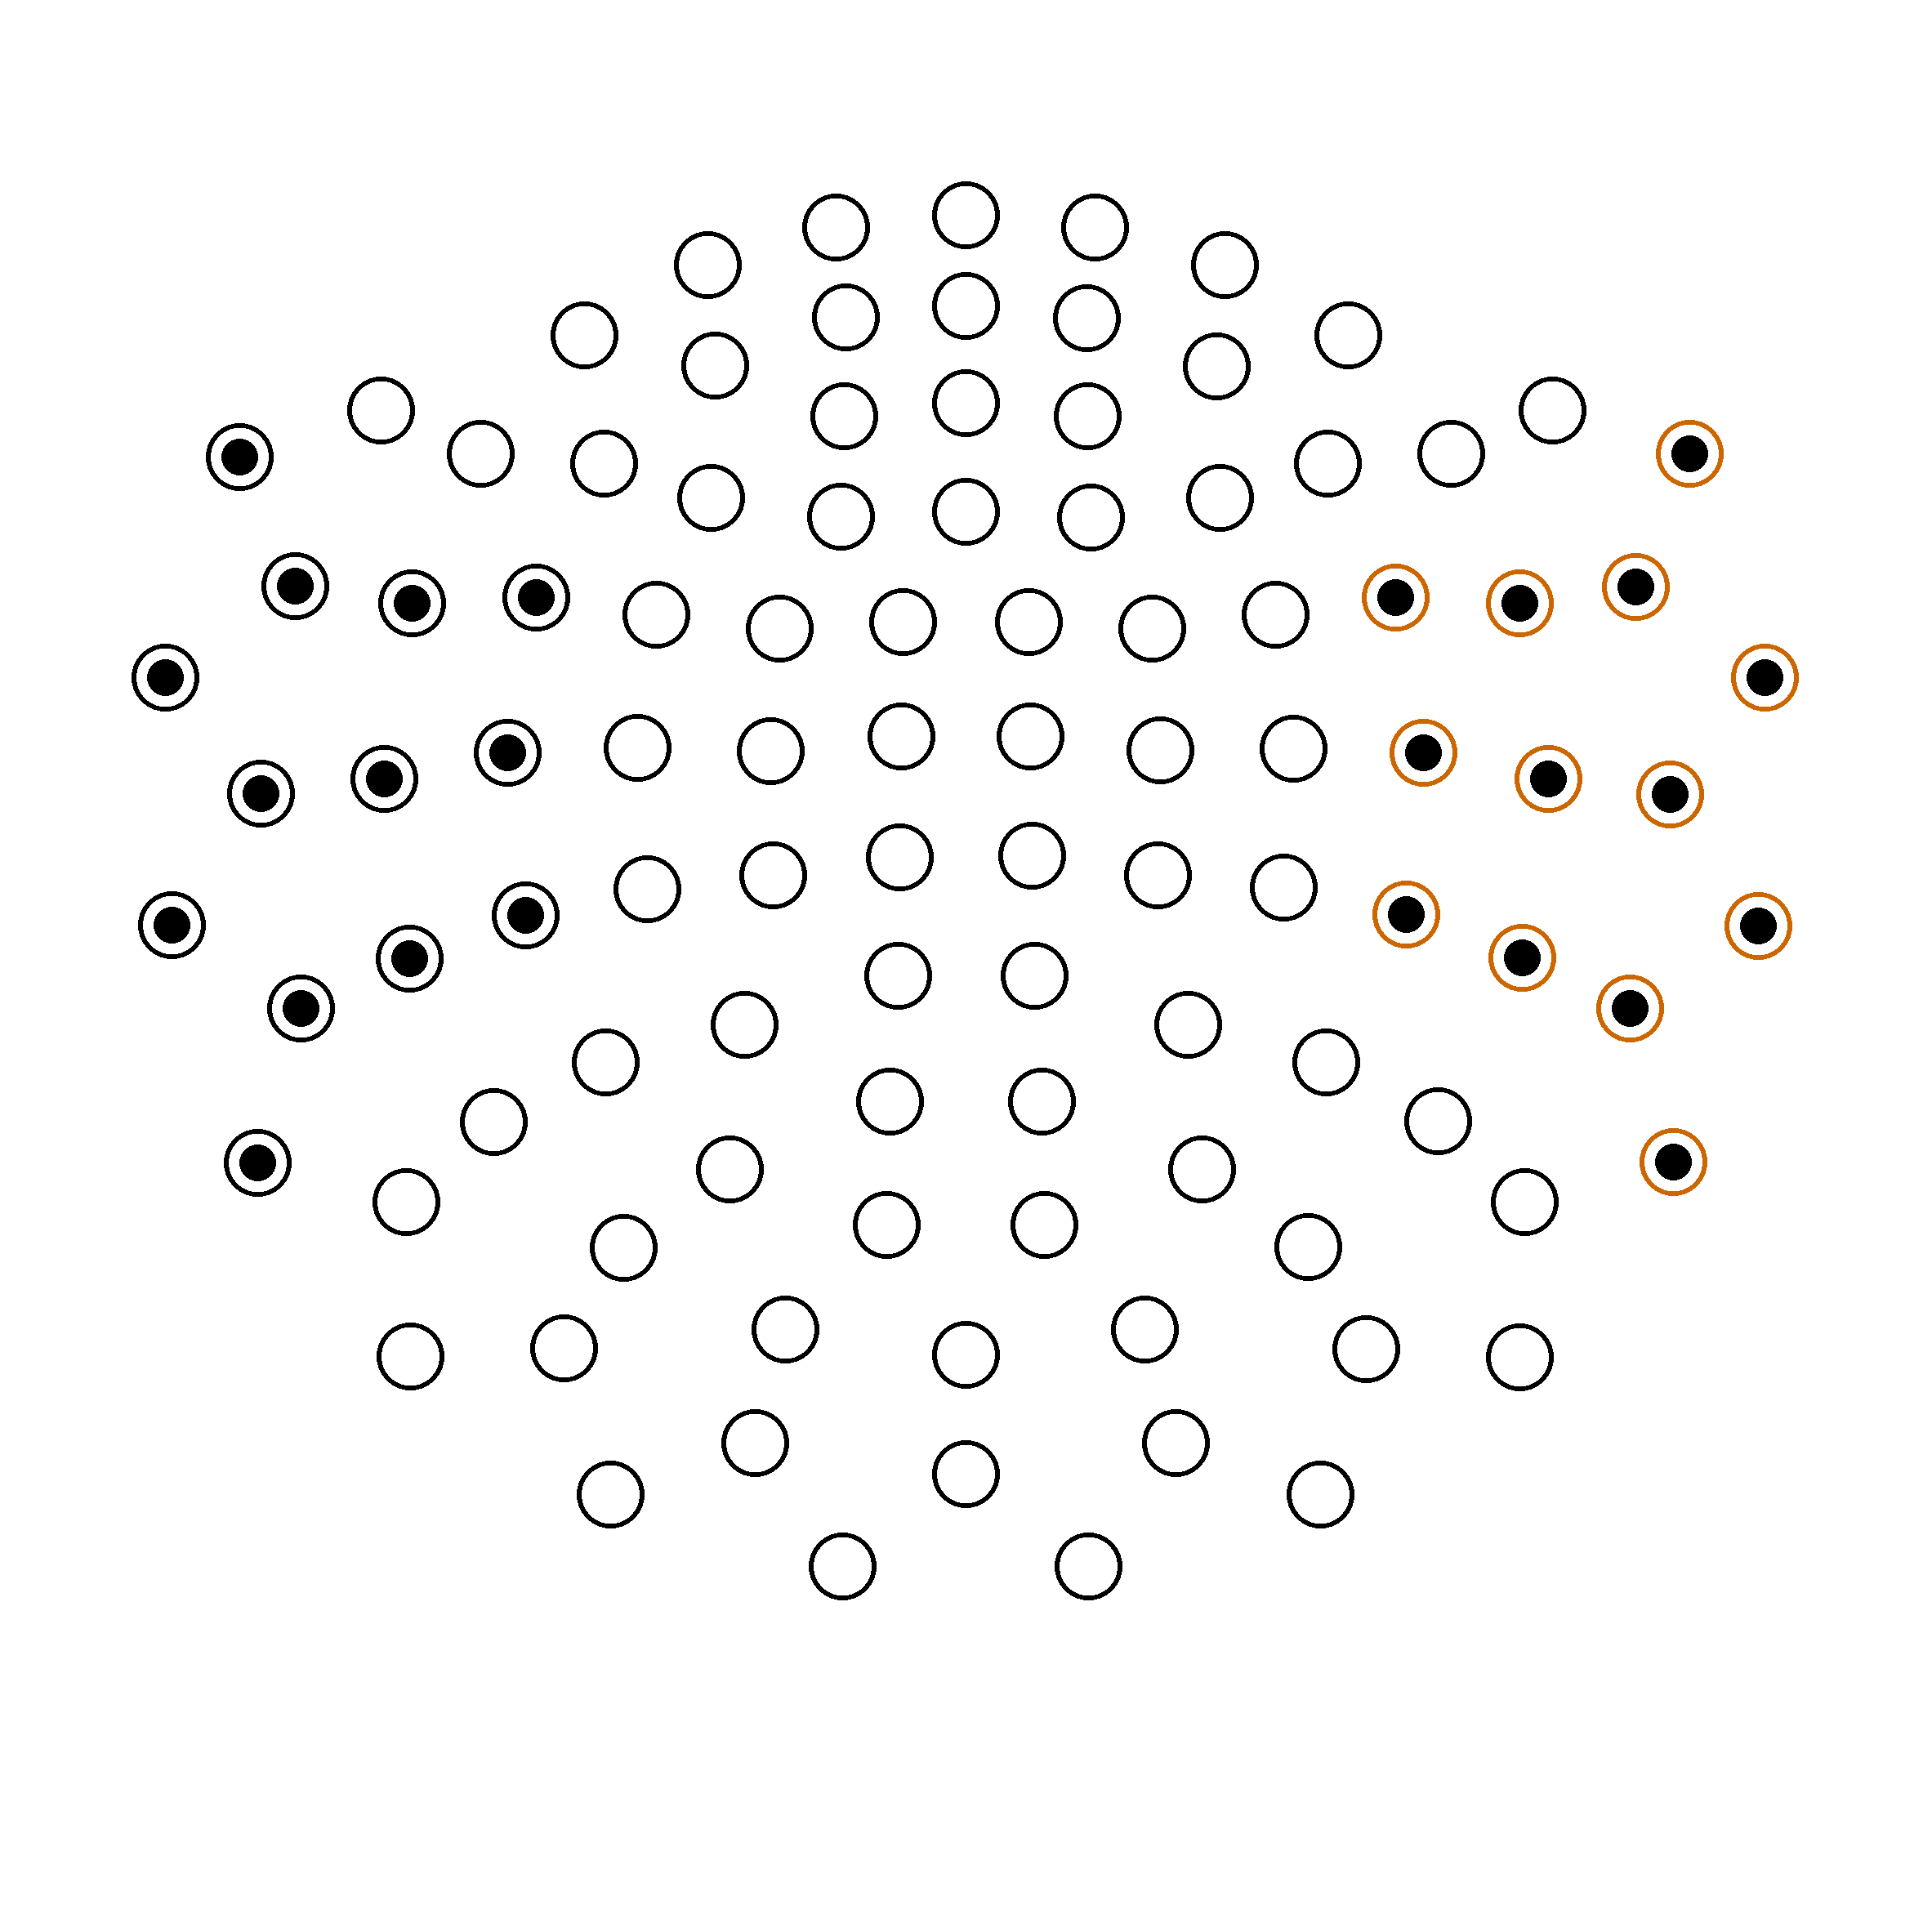
\includegraphics[width=0.24\textwidth]{pics/3_3_temporal_sensors}
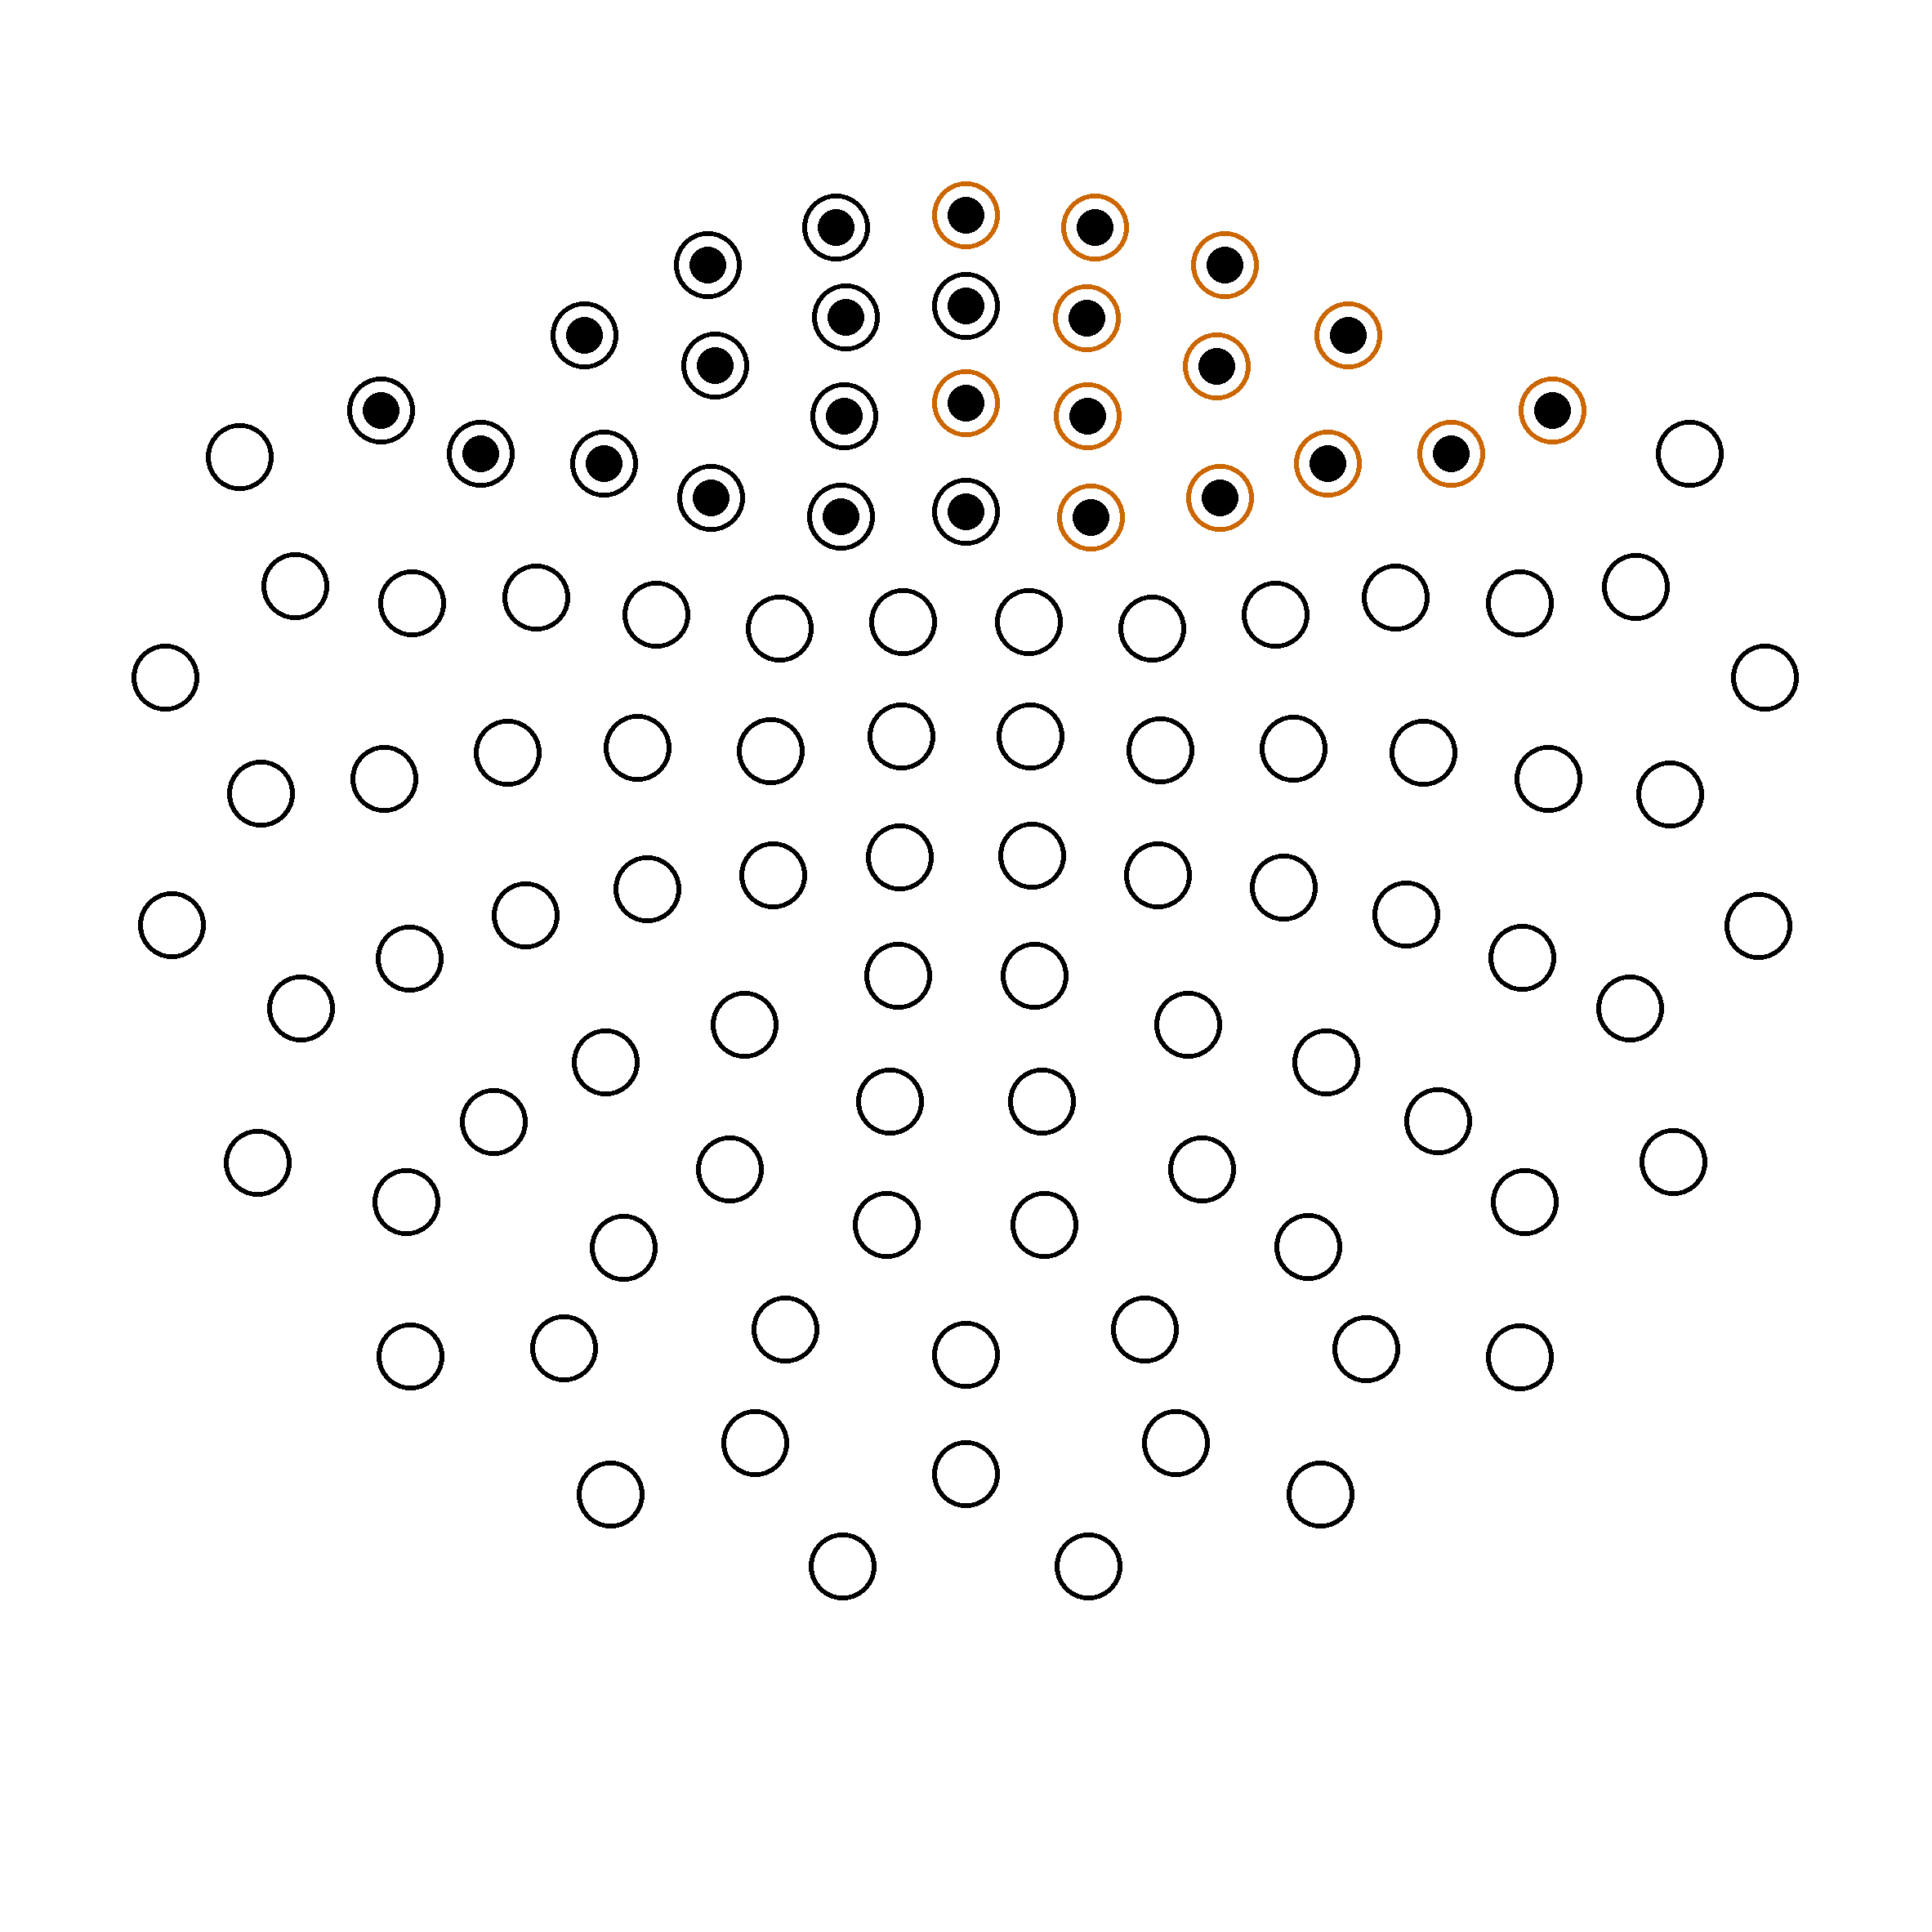
\includegraphics[width=0.24\textwidth]{pics/3_3_frontal_sensors}
\caption{\label{3.3.sensors} Selected channels for each sensor location. From left to right: occipital, parietal, temporal, frontal. The right hemisphere (in red) is also depicted on the right side in each illustration.}
\end{center}
\end{figure}

\subsection{Source space activity}

\paragraph{Anatomical preprocessing}
Cortical reconstruction and volumetric segmentation was performed with the Freesurfer image analysis suite, which is documented and freely available for download online (\emph{http://surfer.nmr.mgh.harvard.edu/}).
The technical details of these procedures are described in prior publications (Dale et al., 1999; Dale and Sereno, 1993; Fischl and Dale, 2000; Fischl et al., 2001; Fischl et al., 2002; Fischl et al., 2004a; Fischl et al., 1999a; Fischl et al., 1999b; Fischl et al., 2004b; Han et al., 2006; Jovicich et al., 2006; Segonne et al., 2004, Reuter et al. 2010, Reuter et al. 2012).
I followed the recommended processing pipeline ("'recon-all"'), with three optional functions.

First, the option "'-nuintensitycor-3T"' improved brain segmentation accuracy by optimizing the bias field correction \cite{3.3.nuintensity}.

Second, by invoking "'-notal-check"', I skipped the Talairach registration checks.
Talairach registration was prone to failure especially in the infant subjects, and uneccessary for our further processing steps.

Third, I supplied and included T2-weighted MRI datasets with the options "'-T2"' and "'-T2pial"'.
The combination of T1- and T2-weighted images improves tissue differentiation especially around the pia mater, yielding a more accurate cortex segmentation.
This pipeline yielded a continuous, antomically plausible cortical surface in MRI space.


\paragraph{Forward and inverse operator}
For the forward operator, three components were necessary: a source model, a BEM model and a coregistration file.

The cortical surface from Freesurfer was used to construct the source model.
Sources were generated by the MNE package \emph{mne\_setup\_bem}.
The result were 20484 sources (10242 per hemisphere), distributed with approximately equal density over the cortical surface.

The head surface from Freesurfer was used to extract a scalp surface layer.
The BEM was constructed from this scalp layer with the MNE package \emph{mne\_surf2bem}, using the default options.
This function sampled down the original surface to the 4th subdivision of an icosahedron.
The finished BEM consisted of 5140 nodes.

Finally, a coregistration file provided the transformation between MRI space and MEG space.
This coregistration attempted to minimize the distance between digitized head surface points and the head surface extracted from the MRI. 
It was performed for each subject individually using the MNE package \emph{mne\_analyze}.
The initial fit was done manually, with visual error feedback.
The following fine adjustment was performed automatically.
This process was repeated until the average spatial error was less than 2mm.
These three components were assembled into a forward operator by the method \emph{mne\_do\_forward\_solution()}.


For the inverse operator, three components were necessary: the forward model, a noise covariance matrix, and a regularization factor.
Each component was calculated individually for each subject.

The first component, the forward model, was supplied by the previous step.

For the second component, the noise covariance matrix, the 1000ms after visual onset were extracted from each trial.
Then, the covariance matrix was computed from this data with the function \emph{mne.compute\_covariance()}.

The third component, the regularization factor was determined from this noise covariance matrix.
First, only coefficients from gradiometer channels were selected.
Second, these coefficients were transformed with a singular value decomposition.
Third, the upper cutoff was defined as the first value of the transformed coefficients.
Fourth, the index at which the transformed coefficients performed the steepest drop in logarithmic value was determined.
Fifth, this index was defined as the maximum amount of usable dimensions.
Sixth, the lower cutoff was defined as the value at this index, plus 15\%.
Seventh, the regularization factor was computed by dividing the lower cutoff by the higher cutoff.


The inverse operator was computed from these three components by the method \linebreak \emph{mne\_do\_inverse\_operator()}. The regularization factor was supplied with the option \linebreak "'--megreg"'.

\paragraph{Inverse solution}
For determining regional cortical activity, 8 regions needed to be defined: the primary auditory cortex (PAC), the anterior and posterior parts of the superior temporal sulcus and gyrus (aSTS, pSTS, aSTG and pSTG), Brodmann area 45 (BA45), Brodmann area 44 (BA44) and the ventral Brodmann area 6 (BA6v).
These regions were spatially defined manually on the cortex of the reference subject.
Freesurfer provided the aparc.a2009s segmentation, which became the basis for this regional selection.
The final regions of interest on the reference brain are visualized in Fig. \ref{3.3.ROI}.
Regions were then mapped from the reference cortex onto the cortices of all other subjects during the next step.

\begin{figure}[h]
\begin{center}
\vspace{7mm}
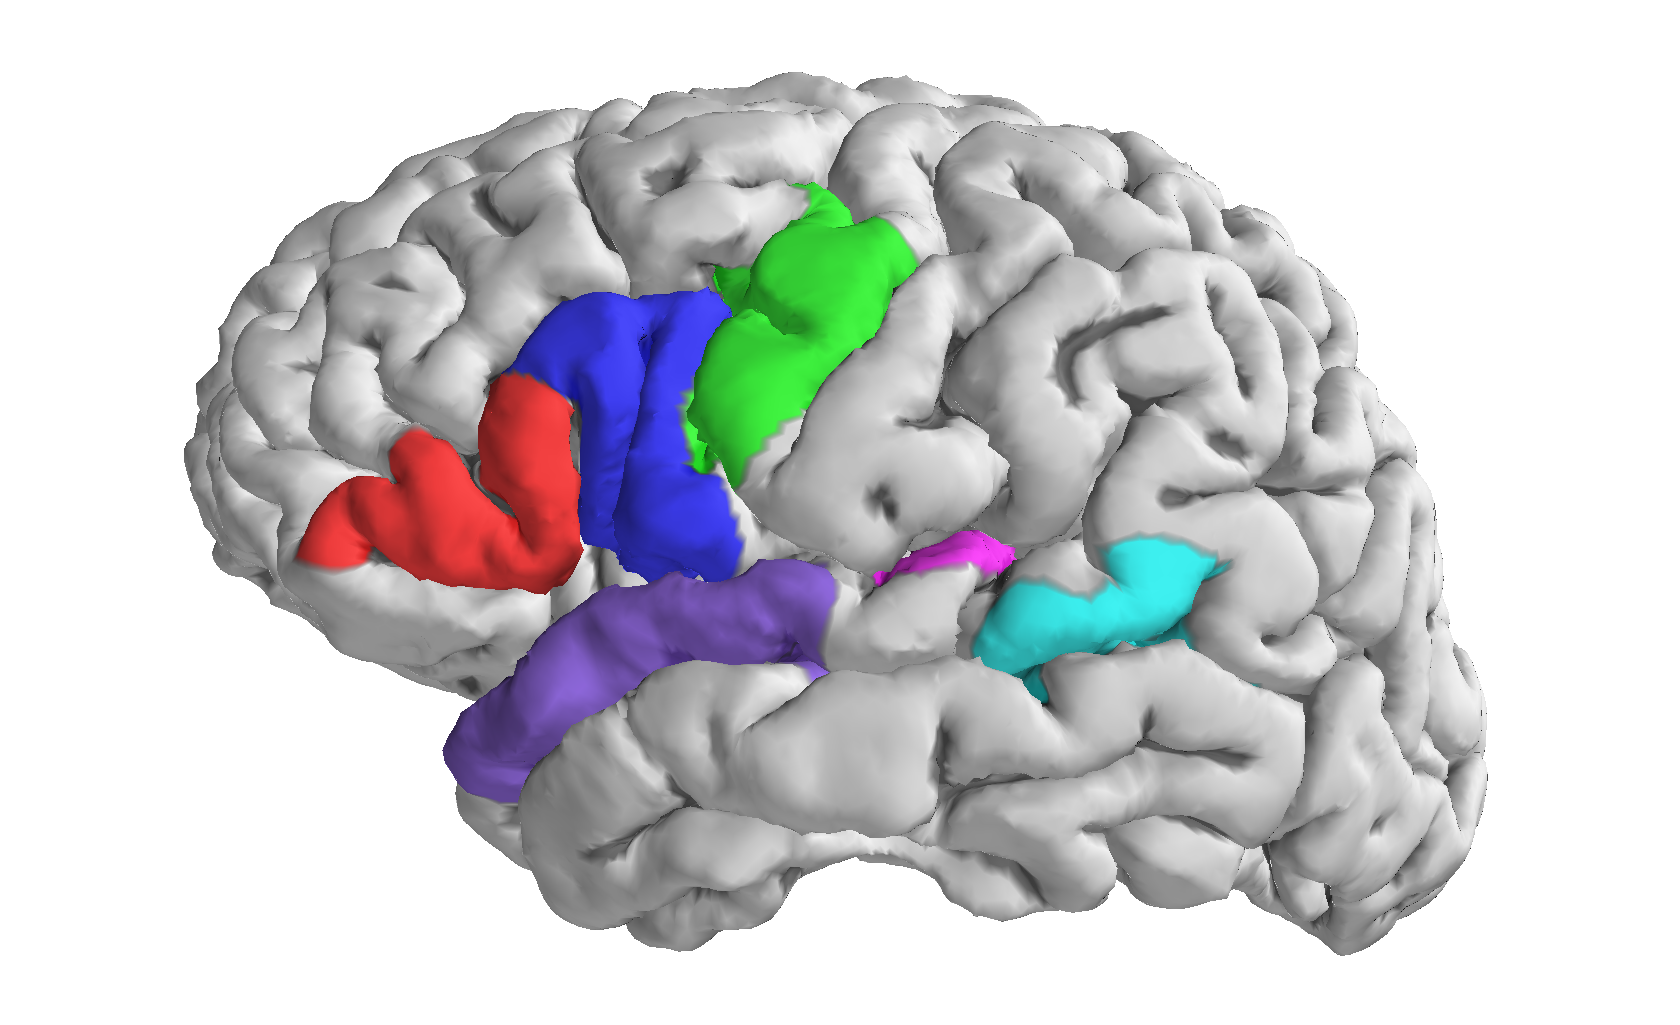
\includegraphics[width=0.49\textwidth]{pics/dh55a-pial-lh}
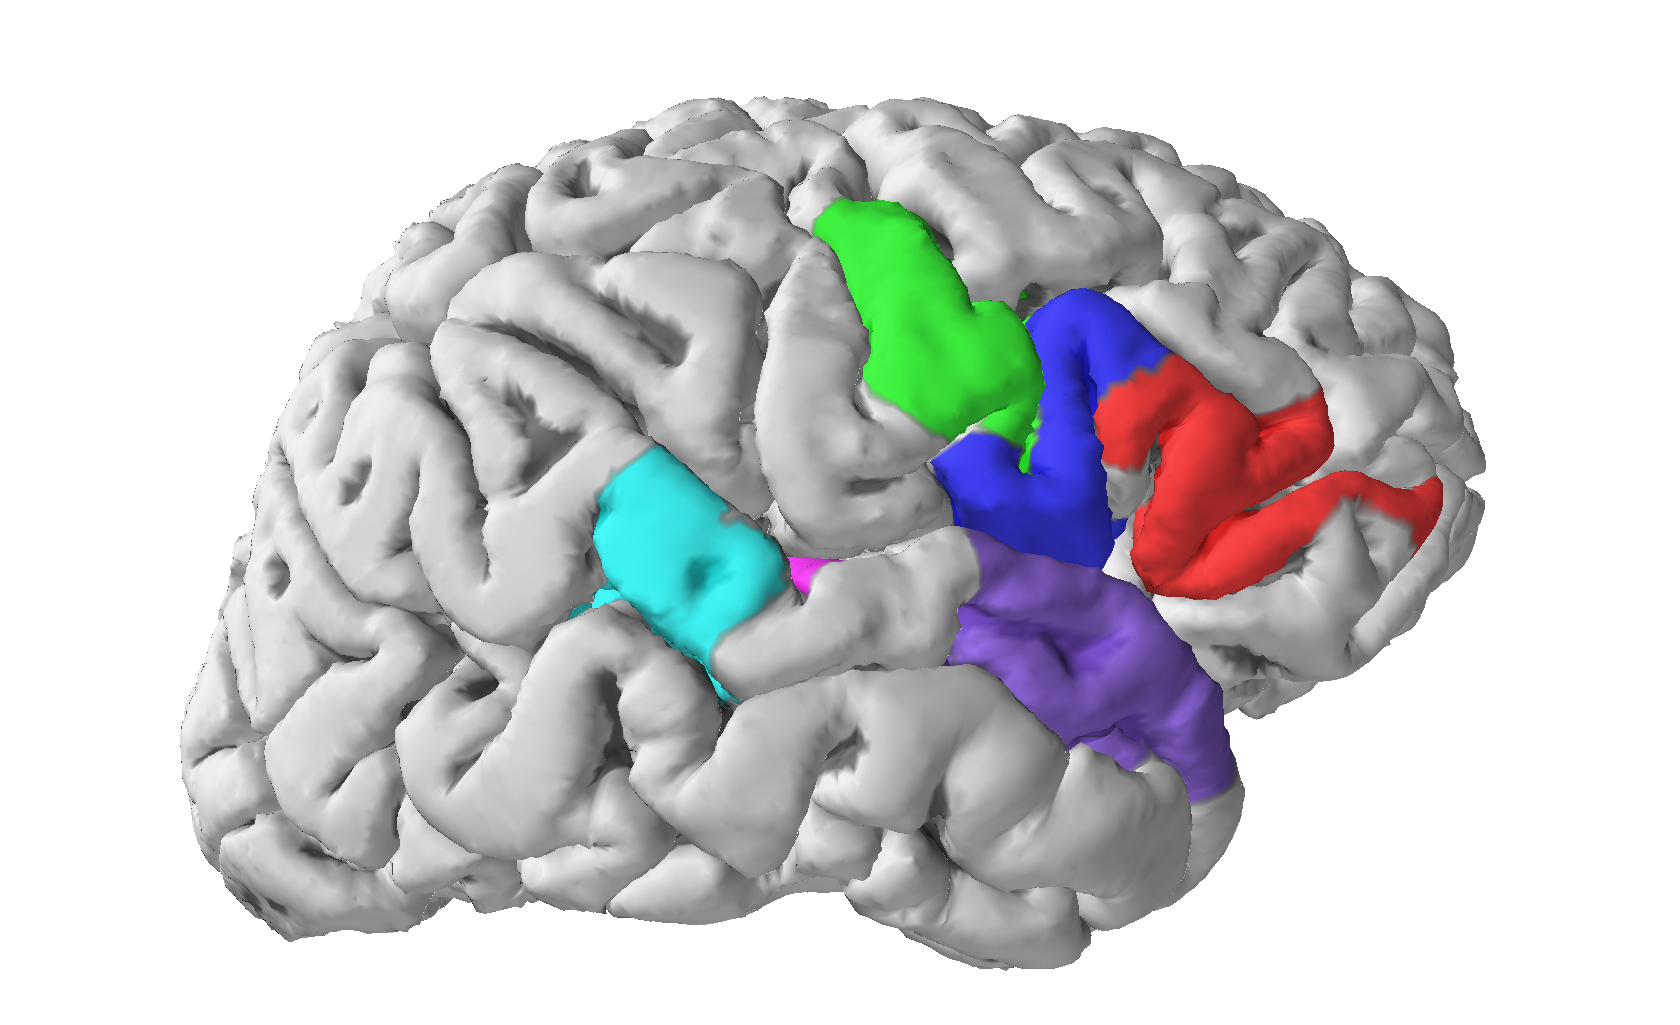
\includegraphics[width=0.49\textwidth]{pics/dh55a-pial-rh}
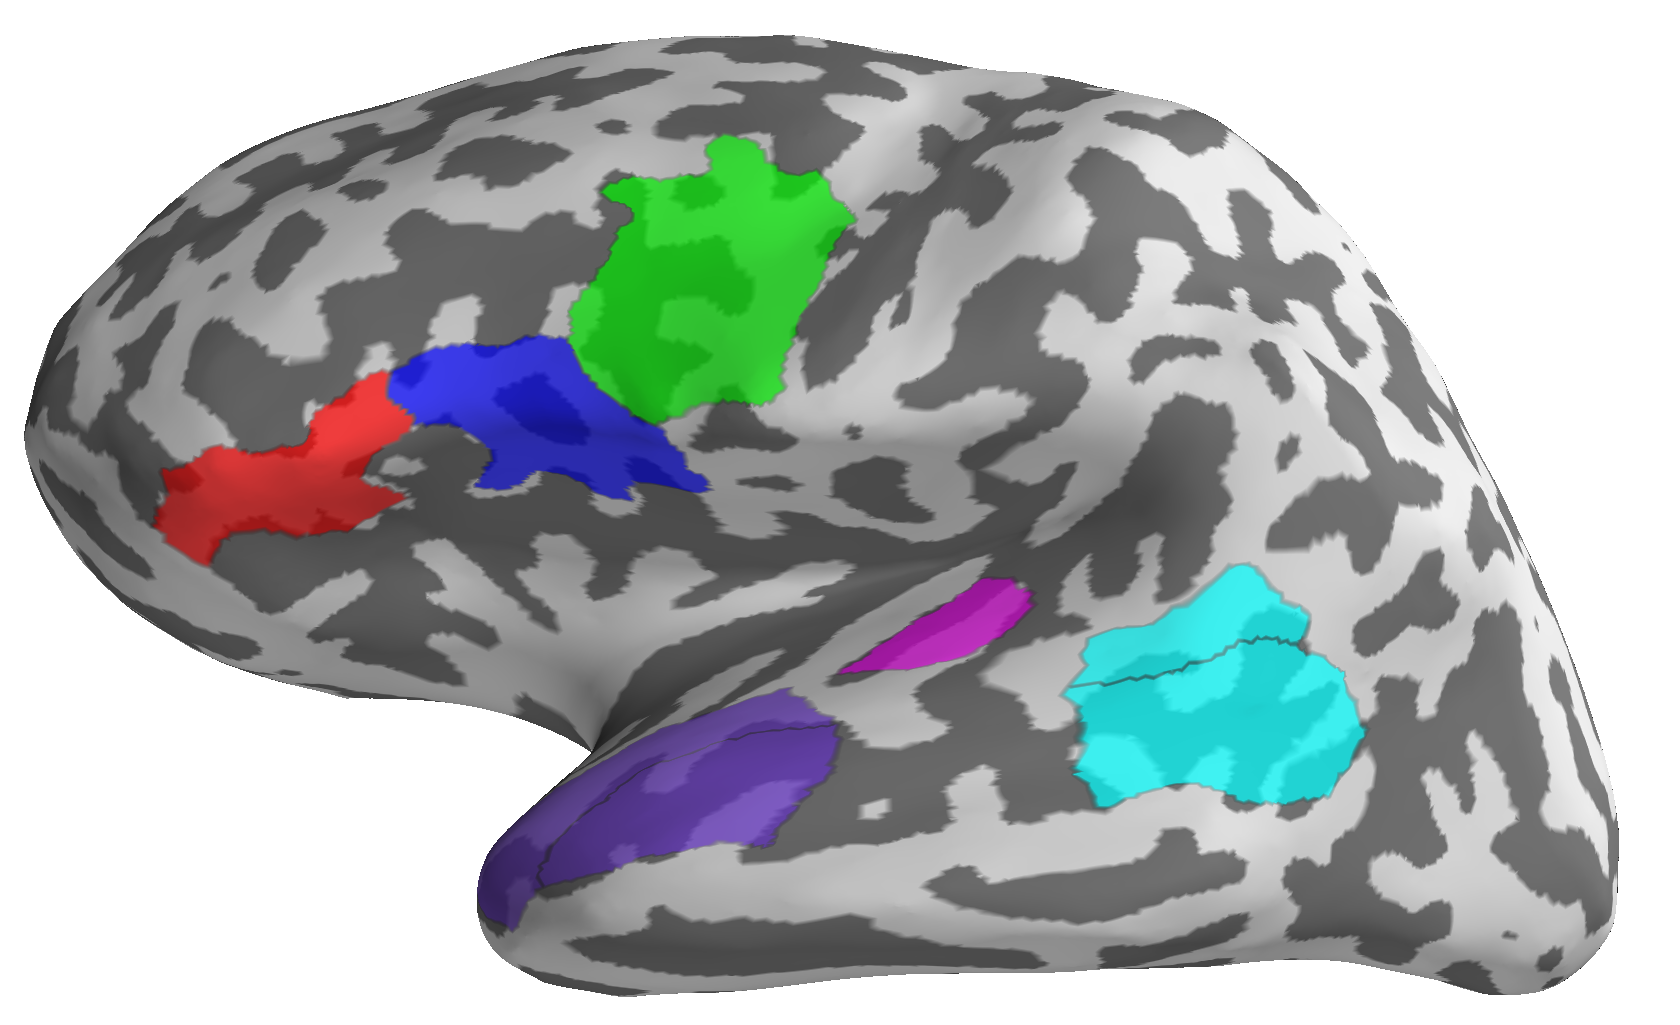
\includegraphics[width=0.49\textwidth]{pics/dh55a-inflated-lh}
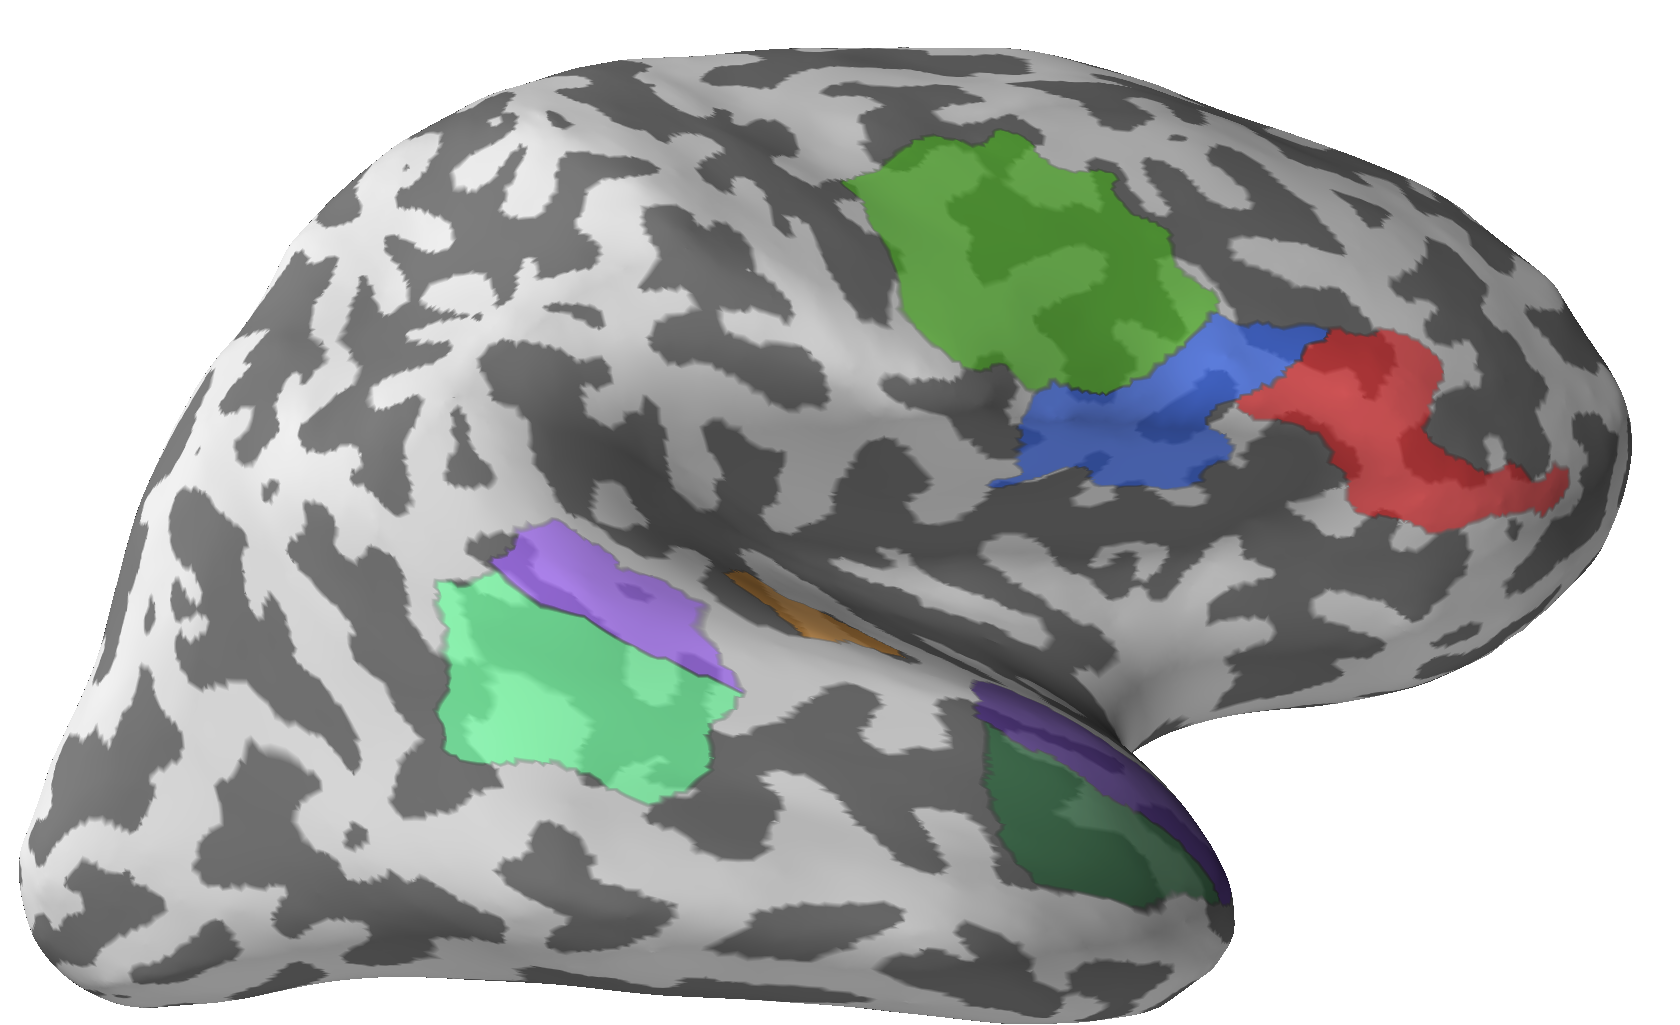
\includegraphics[width=0.49\textwidth]{pics/dh55a-inflated-rh}
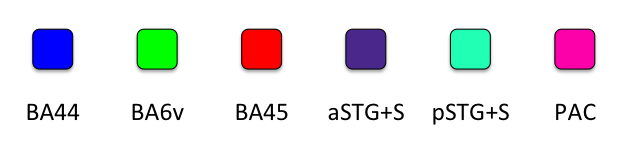
\includegraphics[width=0.75\textwidth]{pics/3_3_ROIlegend}
\caption{\label{3.3.ROI} Selected regions of interest on the reference brain. Top: selected regions on the folded cortex. Bottom: selected regions on the inflated cortex.}
\end{center}
\end{figure}

The inverse operator was then used to calculate inverse solutions from MEG sensor data.
Inverse solutions were calculated for each time point, region, trial and subject individually.
The process was performed by the function \emph{mne.minimum\_norm.apply\_inverse\_epochs()}, with sLORETA as the inverse method.
The option "'pick\_ori=normal"' designated currents leaving and entering the cortex as positive and negative, respectively.
Due to the combination of passive and active noise reduction and artifact suppression, I assumed a fairly high signal-to-noise-ratio (SNR) of 50:1 for each individual source.
The regularization factor was estimated by $\frac{1}{SNR} = 2.5*10^{-3}$.
The result was a series of activation patterns within each region.
Finally, the mean of regional node activity was calculated for each time point, region, trial and subject.


The resulting localized activity was subjected to a cluster analysis.
Extracted trials were pooled over all subjects within a group.
Within each group, two sets of trials were created from the two syntax conditions.
Each trial contained mean activity from eight regions (PAC, aSTS, aSTG, pSTS, pSTG, BA44, BA45 and BA6v).
Clusters were determined by running the MNE function $stats.permutation\_cluster\_test()$ \cite{3.3.clustertest} over the two sets of trials.
The function was run with 2500 permutations, and an t-threshold of 2.0.
The results from each group was evaluated separately.

Additionally, a blind comparison was performed for sensor activity in a series of time intervals.
10 time intervals were established from 0ms to 2200ms after onset, spanning 200ms each.
The mean activity was computed for each region (8), hemisphere (2), and time interval (10), yielding 160 activity values for each subject and condition.
The corresponding values were pooled over all subjects within each of the two groups, and compared between syntax conditions with a paired Student's T-test.
Results from each hemisphere and region were adjusted with the false discovery rate correction (10 comparisons).

For visualization purposes, grand average activity was calculated for each cortical region, group and condition.


\subsection{Interaction analysis}

The TRENtool software (version 3.3.1, February 2015) was used for exploring entropy transfers between cortical areas.
For this purpuse, data was prepared for each subject individually.
The procedure took place in three sections.


During the first section, the input datasets were prepared.
The preparation required three components: regional activity from single trials, a list of regional comparisons and a set of parameters.

For the first component, two sets of single trials were selected from each subject.
Mean regional activity were then extracted from each trial.
Cortical regions were selected if they showed syntax effects either in the cluster analysis or the interval analysis.
This process yielded six relevant cortical regions: PAC, aSTG, pSTS, BA44, BA45 and BA6v.

For the second component, I selected only the most relevant functional connections between cortical regions.
There are 720 unique possiblities to compare these regions, which would overwhelm\footnote{The comparison over one pair of cortical regions (in forward and reverse directions, over two conditions) required a computation time of 4 hours per subject and timewindow. Calculating transfer entropy between 36 pairs of regions took a total of 70 hours. The task of computing 720 comparisons would take two months - a sufficient reason to switch a GPU-based algorithm\cite{3.4.gpuTE}.} my computational capacities, I limited the comparisons to regions connected along an axonal fiber bundle.

Comparisons between these regions were performed for all regions along three pathways (see Fig. \ref{3.4.regions}).
The regions associated to each pathway are derived from \cite{3.4.pathways}.
First, PAC and pSTG showed effects across both hemispheres.
Therefore, I included comparisons across hemispheres between the mirrored regions (two connections: $PAC_{lh} \rightarrow PAC_rh$ and $pSTG_{lh} \rightarrow pSTG_rh$).
Whenever PAC or pSTG were involved in a pathway, I included the regions from both hemispheres.
The primary dorsal pathway connects PAC and BA6v, yielding two connections ($PAC_{lh} \rightarrow BA6v_{lh}$ and $PAC_{rh} \rightarrow BA6v_{lh}$).
The secondary dorsal pathway connects PAC, pSTG and BA44, yielding six unique connections ($PAC_{lh} \rightarrow pSTG_{lh}$, $PAC_{lh} \rightarrow pSTG_{rh}$, $PAC_{rh} \rightarrow pSTG_{lh}$, $PAC_{rh} \rightarrow pSTG_{rh}$, $pSTG_{lh} \rightarrow BA44_{lh}$ and $pSTG_{rh} \rightarrow BA44_{lh}$).
The ventral pathway connects PAC, aSTG and BA45, yielding three unique connections ($PAC_{lh} \rightarrow aSTG_{lh}$, $PAC_{rh}-aSTG_{lh}$ and $aSTG_{lh} \rightarrow BA45_{lh}$).
Since BA44 and BA45 are direct neighbors, their connections ($BA44_lh \rightarrow BA45_lh$) was included too.
Finally, the end points of secondary dorsal and ventral tract were added to the comparison, yielding four connections in total ($PAC_{lh} \rightarrow BA44_{lh}$, $PAC_{rh} \rightarrow BA44_{lh}$, $PAC_{lh} \rightarrow BA45_{lh}$ and $PAC_{rh} \rightarrow BA45_{lh}$).
The reverse direction was added for each of these 18 comparisons, yielding 36 pair-wise comparisons in total.

\begin{figure}[h]
\begin{center}
\vspace{7mm}
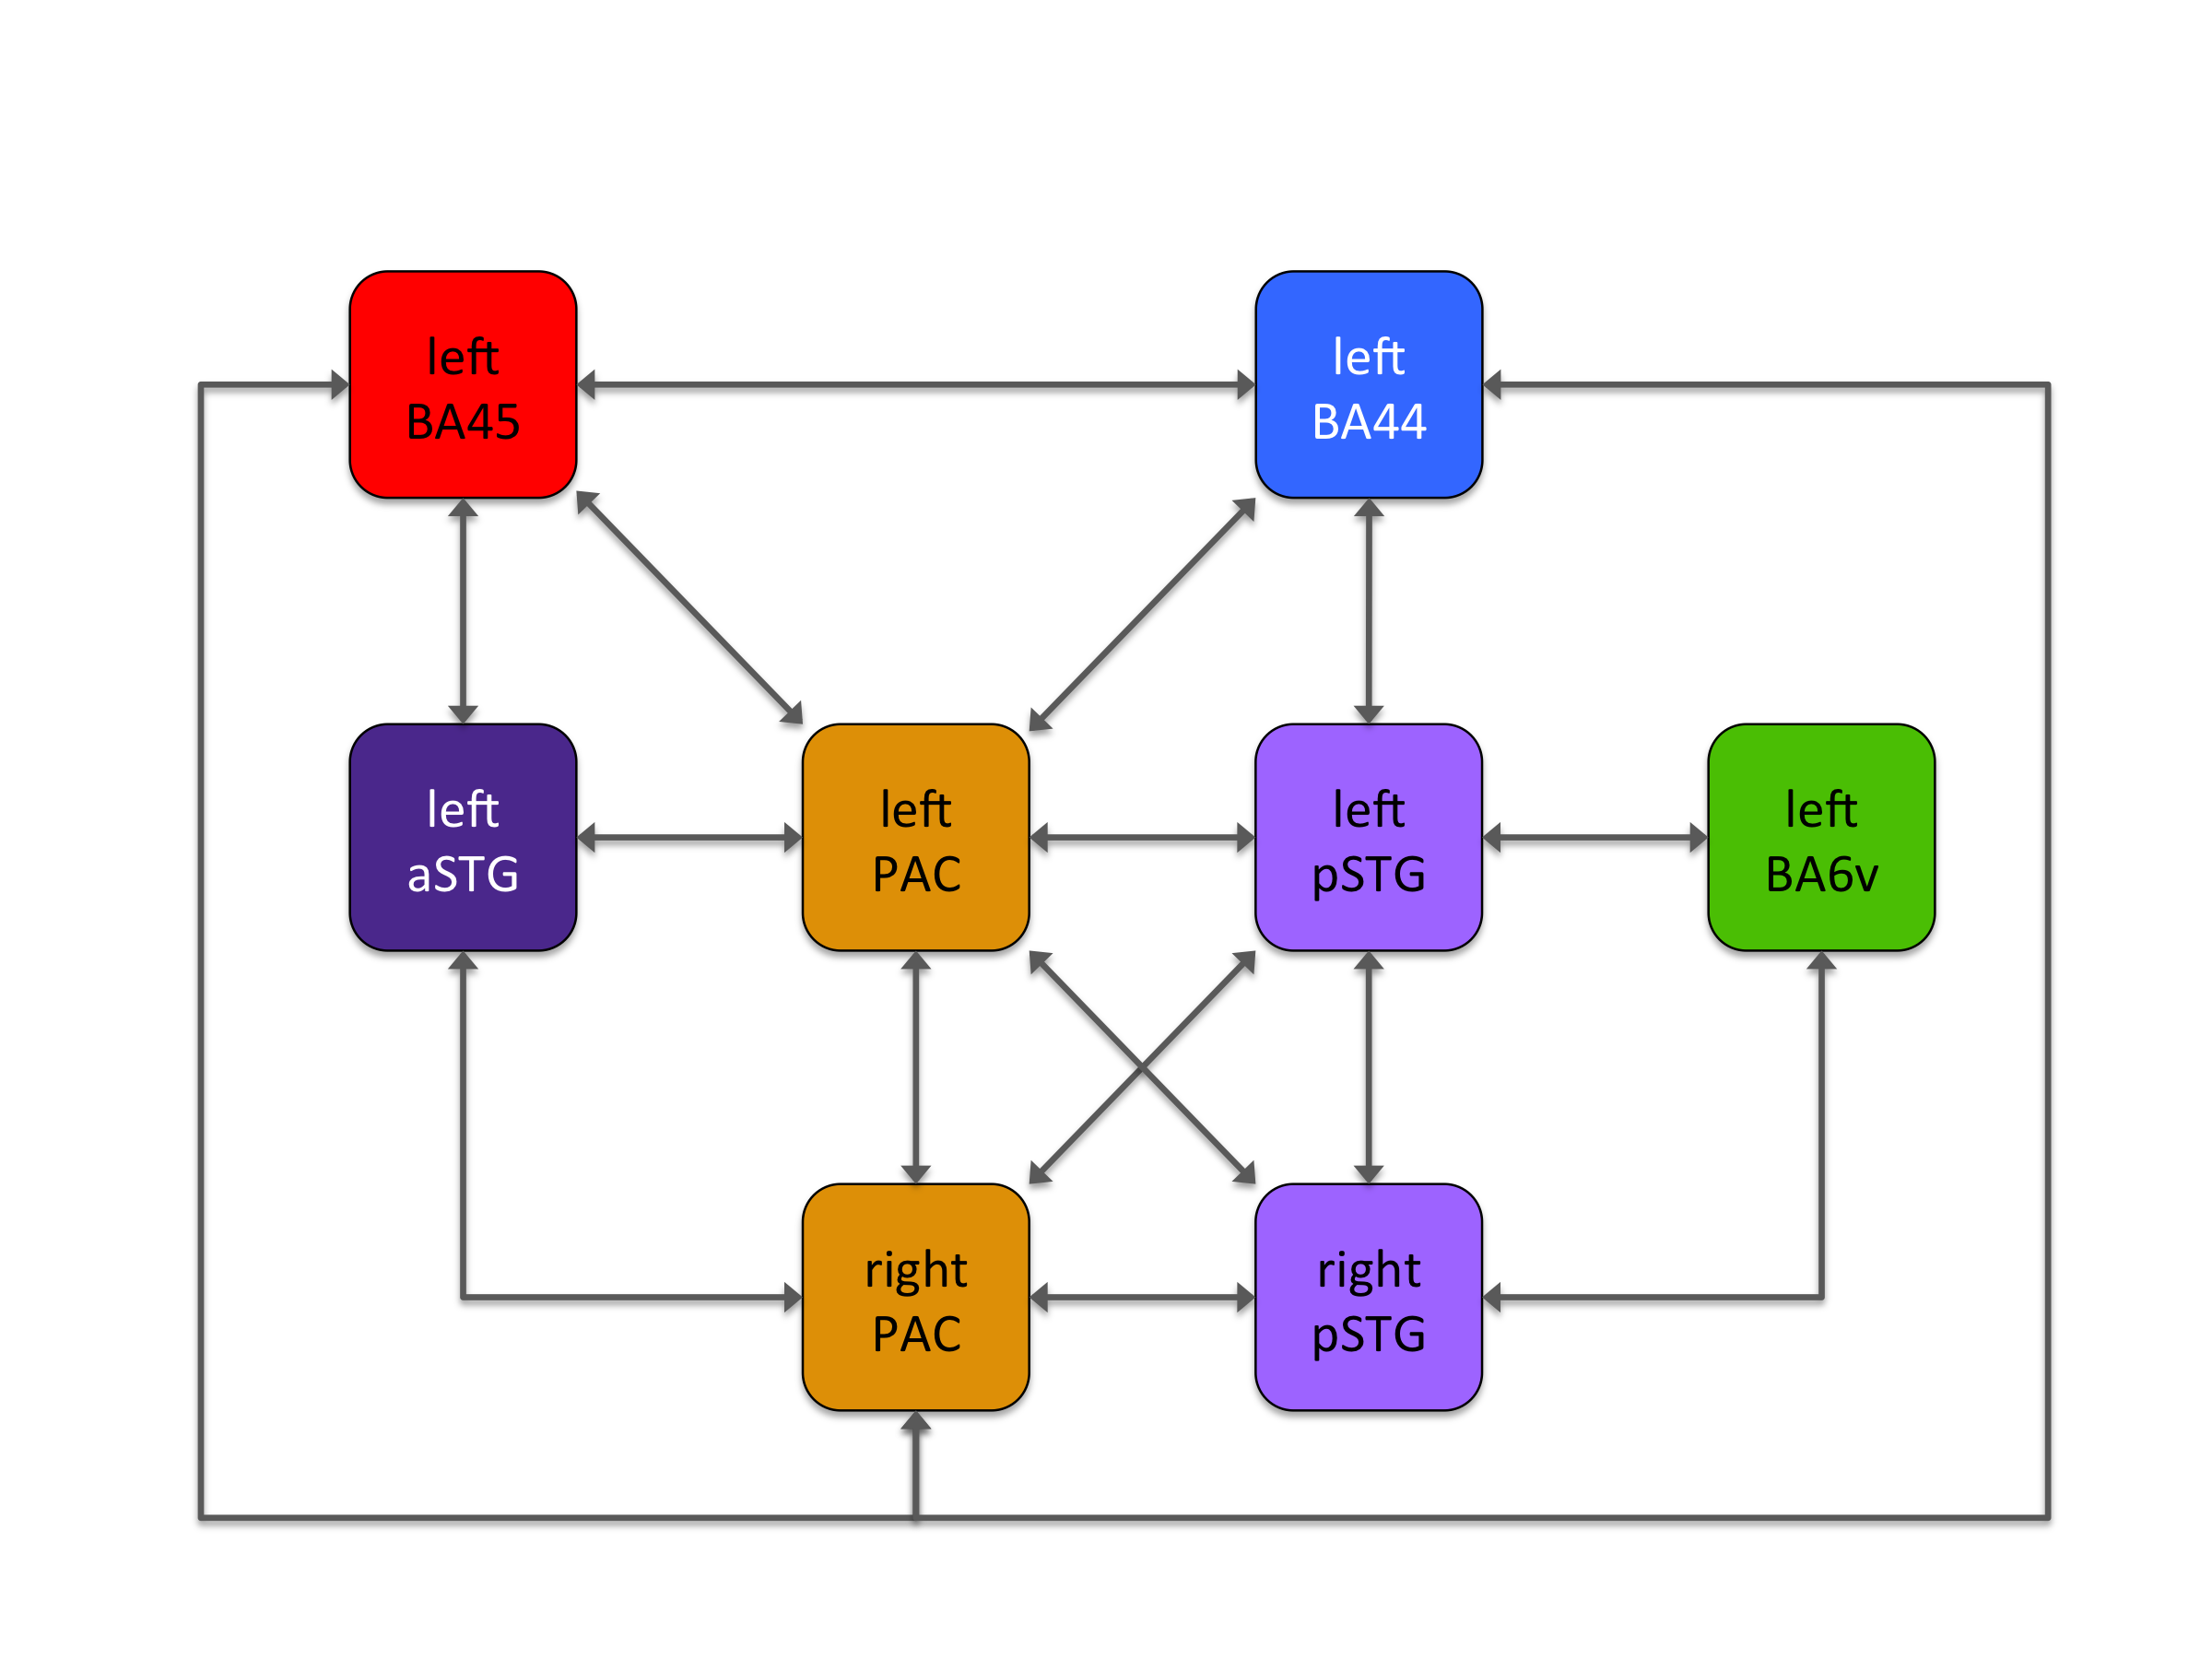
\includegraphics[width=0.75\textwidth]{pics/3_4_regions.png}
\caption{\label{3.4.regions} Connections of selected cortical regions for the computation of transfered entropy. Left of PAC: ventral pathway; top left of PAC: primary dorsal pathway; right of PAC: secondary dorsal pathway.}
\end{center}
\end{figure}

The third component concerned a set of parameters for the data preparation.

The interval analysis yielded (see chapter \ref{4.3}) three distinct time intervals with syntax effects: 0ms - 300ms, 400ms - 800ms and 1000ms - 1600ms.
I supplied those intervals for the estimation of transfer entropy with the parameter \emph{cfg.toi} in three subsequent analyses.

The transfer entropy estimation fundamentally relies on the comparison between two probability density functions.
These mathematical constructs can only be approximated by using scalar time series.
For this purpose, time series from individual trials were combined into a multidimensional state space by TrenTOOL.
This multidimensional space was then reduced into probability density function in a process called embedding.
For optimizing the embedding procedure, I selected the Ragwitz criterion (\emph{cfg.optimizemethod = 'ragwitz'}).
The parameters were supplied as ranges: the relative embedding delay \emph{cfg.ragtaurange = 0.15:0.3} and the embedding dimension \emph{cfg.ragdim = 2:8}.

For the embedding process, a considerable section of data is necessary to estimate the baseline entropy before the interaction time cue occurs.
This section of data is referred to as embedding delay, and won't be included in the analysis of transfer entropy.
The required embedding delay for this combination of data and embedding parameters was 753ms.
I extended the lower time limit of each analysis time window by the same amount.
The Ragwitz criterion then optimized the embedding parameters for each set of time series (once per subject, time window and condition).
The most common optimal embedding dimension was 8, and the mean optimal relative embedding delay was 0.2.

Finally, the parameter \emph{cfg.repPred} indicated the amount of samples that would be used for the interaction analysis.
I maximized this value by calculating \emph{cfg.repPred = sampleLength - embeddingDelay - 1}, with \emph{sampleLength} as the amount of samples in the selected time window and \emph{embeddingDelay}\footnote{Unfortunately, TrenTOOL doesn't display the embedding delay. The formula I used to calculate it is, in Matlab notation, \emph{(max(cfg.ragdim)-1) $\cdot$ max(cfg.ragtaurange) + cfg.predicttimemax\_u + max(ACT)}. \emph{ACT} (the delay for the first minimum of the autocorrelation), in turn, is only computed during the preprocessing phase. Due to time constraints, I opted for a manual approach. An error message printed the current \emph{max(ACT)} if \emph{cfg.repPred} was too small, so I could supply this value into the configuration variable and re-run the preprocessing phase. After a few iterations, the absolute maximum ACT was found, allowing me to adjust the time windows and finish the preprocessing phase.} the amount of samples in the absolute embedding delay.
This is the largest possible value that doesn't violate the assumptions behind the transfer analysis algorithm.


During the second section, TrenTOOL performed a interaction shift test.
This procedure (performed with the function \emph{InteractionDelayReconstruction\_calculate()}) counteracts bias introduced by noise, for example the common false positive detection of an interaction from a less noisy to a more noisy data set.
The shift test establishes the optimal delay of transfered entropy for each comparison of activity.
Transfer entropy was computed for a time range of possible interaction delays: 1ms to 40ms in steps of 5ms.
TrenTOOL then selected the interaction delay with the biggest associated transfer entropy as the most likely representation of the signal delay caused by cognitive processes and anatomic constraints.
To alleviate issues with volume conduction, I supplied the option \emph{cfg.extracond = 'Faes\_method'}.
Unfortunately, using this method prevents the determination of the precise signal delay.
Since the signal delay is not relevant to my research goals, this trade-off was trivial to solve.
The optimal dimension for each data set was considered with the option \emph{cfg.optdimusage = 'indivdim'}.
For significance testing, TrenTOOL creates surrogate data.
This data was created by shuffling existing trials (\emph{cfg.surrogatetype = 'trialshuffling'}).
The significance level for this procedure was \emph{cfg.alpha = 0.05}.
I used t-values to represent the statistical results of the shift test (\emph{cfg.permstatstype = 'indepsamplesT'}).
These results indicate the likelihood if an entropy transfer has occurred between the selected pair of regional activity.


The third section evaluated the impact of the syntax condition on the whole group.
For this purpose, a comparison was conducted between conditions over all subjects within a group.
